% ARCHIVO GENERADO por experiments/report.py -- no editar a mano.
% Corrida: 20261126-104206

\subsubsection{Entorno}

\begin{table}[htbp]
\centering
\small
\resizebox{\ifdim\width>\linewidth\linewidth\else\width\fi}{!}{%
\begin{tabular}{|c|c|}
\hline
\textbf{Dato} & \textbf{Valor} \\ \hline
Fecha & 2026-11-26 10:42:06 \\ \hline
Entorno & 3 computadores en red local \\ \hline
Nodos & nodo-01 (172.25.4.83), nodo-03 (172.25.5.66), nodo-02 (172.25.7.119) \\ \hline
Equipo que ejecutó los experimentos & MSI (Windows-11-10.0.26200-SP0) \\ \hline
CPU / RAM de ese equipo & 12 hilos / 15.7 GB \\ \hline
Python & 3.13.7 \\ \hline
Estrategia por defecto & weighted\_load \\ \hline
Tamaño de tarea (puntos Monte Carlo) & 12,000,000 \\ \hline
Modo & completo \\ \hline
\end{tabular}}
\caption{Entorno de la corrida experimental.}
\label{tab:entorno}
\end{table}

Los experimentos se ejecutaron en \textbf{tres computadores físicos} conectados a la misma red local, un nodo por computador.

\subsubsection{Latencia de comunicación}

\begin{table}[htbp]
\centering
\small
\resizebox{\ifdim\width>\linewidth\linewidth\else\width\fi}{!}{%
\begin{tabular}{|c|c|c|c|c|c|}
\hline
\textbf{Nodo} & \textbf{Ping medio (ms)} & \textbf{Ping mín (ms)} & \textbf{Ping máx (ms)} & \textbf{Tarea mínima p50 (ms)} & \textbf{Tarea mínima p95 (ms)} \\ \hline
nodo-02 & 61.116 & 30.221 & 136.877 & 7.733 & 26.384 \\ \hline
nodo-03 & 24.971 & 16.617 & 38.265 & 9.414 & 21.802 \\ \hline
\end{tabular}}
\caption{Latencia hacia cada nodo.}
\label{tab:latencia}
\end{table}

\emph{Ping} es el RTT de los mensajes \texttt{PING}/\texttt{PONG} que cada nodo mide a sus vecinos. \emph{Tarea mínima} es el tiempo completo de una tarea \texttt{echo} (asignación, envío, ejecución y respuesta).

\begin{figure}[htbp]
\centering
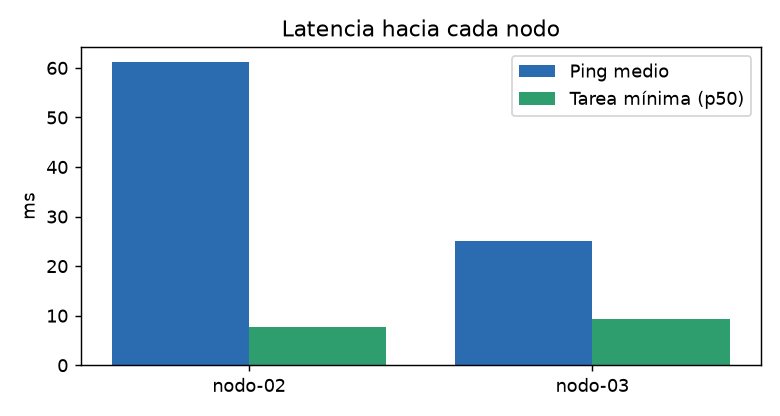
\includegraphics[width=0.7\textwidth]{figuras/latencia.png}
\caption{Latencia hacia cada nodo.}
\label{fig:latencia}
\end{figure}

\subsubsection{Tiempo de descubrimiento}

Se arranca un nodo nuevo, sin conocer a nadie, y se mide el tiempo hasta que descubre a todos los demás.

\begin{table}[htbp]
\centering
\small
\resizebox{\ifdim\width>\linewidth\linewidth\else\width\fi}{!}{%
\begin{tabular}{|c|c|c|c|}
\hline
\textbf{Intento} & \textbf{Segundos} & \textbf{Vecinos encontrados} & \textbf{Completo} \\ \hline
1 & 30.034 & 2 & no \\ \hline
2 & 30.038 & 2 & no \\ \hline
3 & 30.043 & 2 & no \\ \hline
4 & 0.203 & 3 & sí \\ \hline
5 & 0.102 & 3 & sí \\ \hline
6 & 0.101 & 3 & sí \\ \hline
7 & 0.102 & 3 & sí \\ \hline
8 & 0.101 & 3 & sí \\ \hline
\end{tabular}}
\caption{Tiempo de descubrimiento de un nodo nuevo.}
\label{tab:descubrimiento}
\end{table}

Descubrimiento completo en 5/8 intentos. En los 5 intentos completos tardó \textbf{0.12 s} de media (mín 0.10 s, máx 0.20 s). En los 3 restantes se agotó el límite de 30 s sin encontrar a todos los vecinos: el \emph{broadcast} UDP no tiene garantía de entrega y en una red Wi-Fi puede perderse; por eso el sistema también admite vecinos semilla por IP (\texttt{--peers}).

\subsubsection{Escalabilidad}

\paragraph{Más nodos, misma carga.} Se ejecuta el mismo lote de 24 tareas restringiendo el número de nodos disponibles.

\begin{table}[htbp]
\centering
\small
\resizebox{\ifdim\width>\linewidth\linewidth\else\width\fi}{!}{%
\begin{tabular}{|c|c|c|c|c|}
\hline
\textbf{Nodos} & \textbf{Tiempo total (s)} & \textbf{$\pm$ $\sigma$} & \textbf{Tareas/s} & \textbf{Aceleración} \\ \hline
1 & 2.621 & 0.26 & 9.26 & 1.0$\times$ \\ \hline
2 & 1.767 & 0.374 & 14.33 & 1.48$\times$ \\ \hline
3 & 1.69 & 0.137 & 14.29 & 1.55$\times$ \\ \hline
\end{tabular}}
\caption{Escalabilidad al aumentar el número de nodos.}
\label{tab:escal-nodos}
\end{table}

\begin{figure}[htbp]
\centering
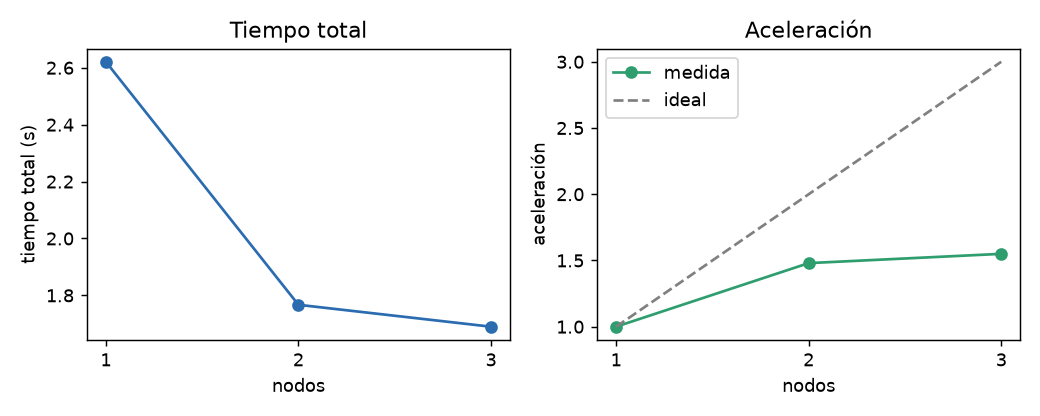
\includegraphics[width=0.9\textwidth]{figuras/escalabilidad_nodos.png}
\caption{Tiempo total y aceleración según el número de nodos.}
\label{fig:escal-nodos}
\end{figure}

Con 3 nodos la aceleración fue \textbf{1.55$\times$} (ideal: 3$\times$). La diferencia con el ideal se debe a la sobrecarga de coordinación (mensajes, ACK), a que las tareas se reparten en bloques discretos y a las diferencias de capacidad entre equipos.

\paragraph{Incremento progresivo de la carga.}

\begin{table}[htbp]
\centering
\small
\resizebox{\ifdim\width>\linewidth\linewidth\else\width\fi}{!}{%
\begin{tabular}{|c|c|c|c|c|c|c|}
\hline
\textbf{Tareas} & \textbf{Tiempo total (s)} & \textbf{Tareas/s} & \textbf{Latencia media (s)} & \textbf{p95 (s)} & \textbf{Tráfico enviado (KB/s)} & \textbf{CPU usada media (\%)} \\ \hline
4 & 0.222 & 17.99 & 0.197 & 0.221 & 6.79 & nodo-01: 24.5, nodo-03: 77.0, nodo-02: 20.2 \\ \hline
8 & 0.454 & 17.61 & 0.286 & 0.453 & 3.92 & nodo-01: 15.7, nodo-03: 77.0, nodo-02: 17.4 \\ \hline
16 & 1.291 & 12.4 & 0.487 & 0.898 & 2.71 & nodo-01: 21.1, nodo-03: 41.8, nodo-02: 17.4 \\ \hline
32 & 2.328 & 13.75 & 1.142 & 2.233 & 4.87 & nodo-01: 14.0, nodo-03: 52.6, nodo-02: 22.4 \\ \hline
64 & 4.417 & 14.49 & 1.455 & 3.801 & 3.57 & nodo-01: 17.3, nodo-03: 28.1, nodo-02: 23.4 \\ \hline
\end{tabular}}
\caption{Respuesta del sistema al aumentar la carga.}
\label{tab:escal-carga}
\end{table}

\begin{figure}[htbp]
\centering
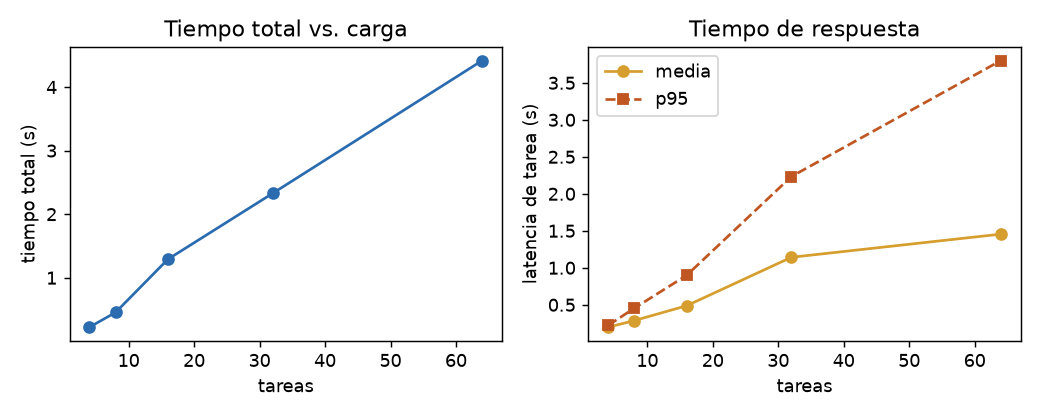
\includegraphics[width=0.9\textwidth]{figuras/carga_progresiva.png}
\caption{Tiempo total y tiempo de respuesta según la carga.}
\label{fig:escal-carga}
\end{figure}

Al multiplicar la carga por 16 (de 4 a 64 tareas) el tiempo total se multiplicó por 19.9 y el rendimiento pasó de 17.99 a 14.49 tareas/s. El tráfico de control fue de 3.57 KB/s con la mayor carga.

\subsubsection{Comparación de estrategias de asignación}

Mismo lote de 36 tareas de tamaño heterogéneo (0.5$\times$, 1$\times$ y 2$\times$) con cada estrategia. \emph{Desbalance} es el coeficiente de variación del número de tareas por nodo (0 = reparto perfecto).

\begin{table}[htbp]
\centering
\small
\resizebox{\ifdim\width>\linewidth\linewidth\else\width\fi}{!}{%
\begin{tabular}{|c|c|c|c|c|c|c|}
\hline
\textbf{Estrategia} & \textbf{Tiempo total (s)} & \textbf{$\pm$ $\sigma$} & \textbf{Latencia media (s)} & \textbf{p95 (s)} & \textbf{Desbalance} & \textbf{Tareas por nodo} \\ \hline
$F(i,j)$ del diseño & 5.029 & 2.334 & 2.621 & 4.929 & 1.414 & nodo-01: 0.0, nodo-02: 24.0, nodo-03: 12.0 \\ \hline
$F(i,j)$ + carga & 3.02 & 0.79 & 1.328 & 2.733 & 0.972 & nodo-01: 9.7, nodo-02: 20.7, nodo-03: 5.7 \\ \hline
Menos cargado & 2.948 & 0.408 & 0.944 & 2.603 & 0.0 & nodo-01: 12.0, nodo-02: 12.0, nodo-03: 12.0 \\ \hline
Menor latencia & 3.365 & 0.087 & 1.701 & 3.275 & 1.414 & nodo-01: 36.0, nodo-02: 0.0, nodo-03: 0.0 \\ \hline
Round-robin & 2.983 & 0.126 & 0.99 & 2.812 & 0.0 & nodo-01: 12.0, nodo-02: 12.0, nodo-03: 12.0 \\ \hline
Aleatoria & 3.078 & 0.34 & 1.011 & 2.855 & 0.203 & nodo-01: 9.7, nodo-02: 12.3, nodo-03: 14.0 \\ \hline
\end{tabular}}
\caption{Comparación de las seis estrategias de asignación.}
\label{tab:estrategias}
\end{table}

\begin{figure}[htbp]
\centering
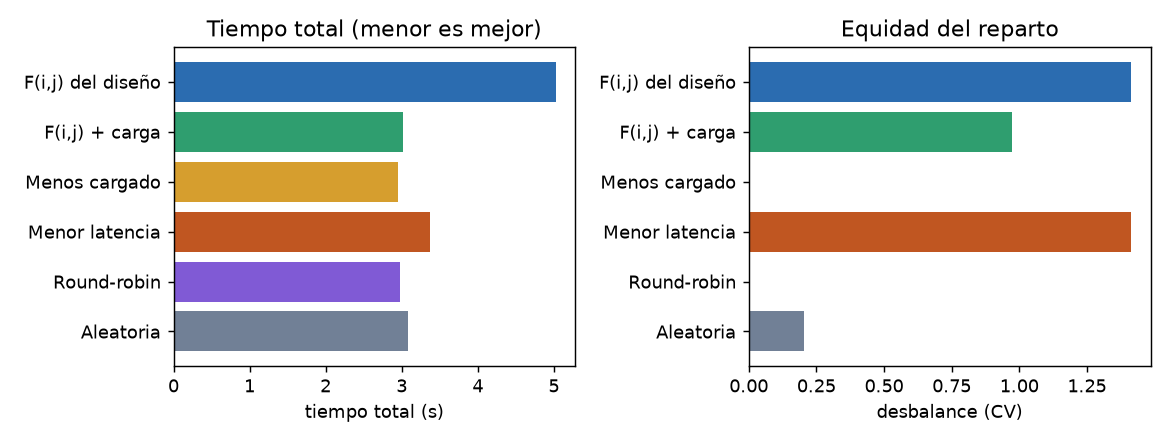
\includegraphics[width=0.9\textwidth]{figuras/estrategias.png}
\caption{Tiempo total y equidad del reparto por estrategia.}
\label{fig:estrategias}
\end{figure}

La estrategia con menor tiempo total fue \textbf{Menos cargado} (2.948 s) y la de mayor tiempo \textbf{$F(i,j)$ del diseño} (5.029 s). La función $F(i,j)$ del diseño original tardó 5.029 s con un desbalance de 1.414. Esa función no considera la carga actual y la normalización min-max convierte diferencias mínimas de CPU y memoria entre nodos desocupados en diferencias de 0 a 1, por lo que puede concentrar tareas en pocos nodos. La variante \texttt{weighted\_load} (término de carga y normalización robusta) redujo el tiempo total en 40\,\% y el desbalance de 1.414 a 0.972, conservando el criterio multicriterio.

\subsubsection{Tolerancia a fallos}

Un nodo cae 2 s después de empezar un lote de tareas (deja de enviar y recibir durante 25 s).

\begin{table}[htbp]
\centering
\small
\resizebox{\ifdim\width>\linewidth\linewidth\else\width\fi}{!}{%
\begin{tabular}{|c|c|c|c|c|c|c|c|c|}
\hline
\textbf{Intento} & \textbf{Nodo caído} & \textbf{Tareas} & \textbf{Completadas} & \textbf{\% completado} & \textbf{Reasignadas} & \textbf{Detección (s)} & \textbf{Recuperación (s)} & \textbf{Tiempo total (s)} \\ \hline
1 & nodo-02 & 20 & 20 & 100.0 & 10 & 4.25 & 4.16 & 10.41 \\ \hline
2 & nodo-03 & 20 & 20 & 100.0 & 4 & 5.38 & 1.22 & 8.61 \\ \hline
3 & nodo-02 & 20 & 20 & 100.0 & 15 & 4.31 & 6.06 & 12.38 \\ \hline
4 & nodo-03 & 20 & 20 & 100.0 & 4 & 4.98 & 1.18 & 8.17 \\ \hline
\end{tabular}}
\caption{Caída de un nodo durante la ejecución de un lote.}
\label{tab:fallos}
\end{table}

\begin{itemize}
\item Detección de la caída: media \textbf{4.73 s} (requisito: $\leq$ 5 s de silencio; la detección corre cada 0.5 s).
\item Tareas completadas pese a la caída: \textbf{100\,\%} (sin intervención manual).
\item La \emph{recuperación} es el tiempo desde la primera reasignación hasta que la tarea reasignada termina (incluye volver a ejecutarla).
\end{itemize}

\begin{figure}[htbp]
\centering
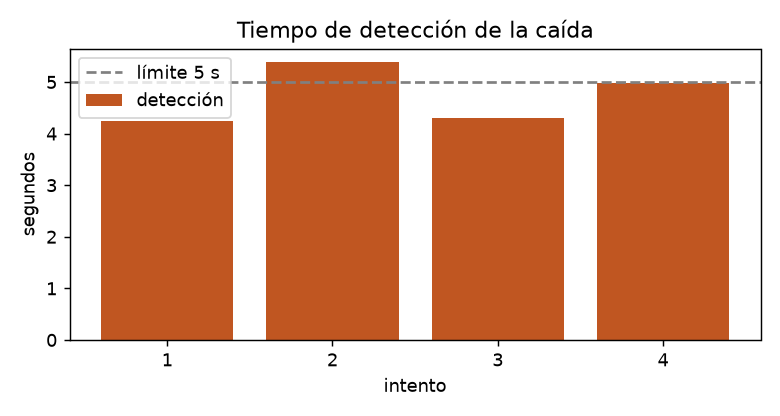
\includegraphics[width=0.7\textwidth]{figuras/tolerancia_fallos.png}
\caption{Tiempo de detección de la caída en cada intento.}
\label{fig:fallos}
\end{figure}

\subsubsection{Disponibilidad del servicio}

Cada 0.5 s se envía una tarea de sondeo mientras nodo-02 falla entre $t = 15$ s y $t = 35$ s.

\begin{table}[htbp]
\centering
\small
\resizebox{\ifdim\width>\linewidth\linewidth\else\width\fi}{!}{%
\begin{tabular}{|c|c|}
\hline
\textbf{Métrica} & \textbf{Valor} \\ \hline
Sondas enviadas & 140 \\ \hline
Completadas & 100.0 \% \\ \hline
Completadas en $\leq$ 3 s & 97.86 \% \\ \hline
\end{tabular}}
\caption{Disponibilidad del servicio durante la falla de un nodo.}
\label{tab:disponibilidad}
\end{table}

\begin{figure}[htbp]
\centering
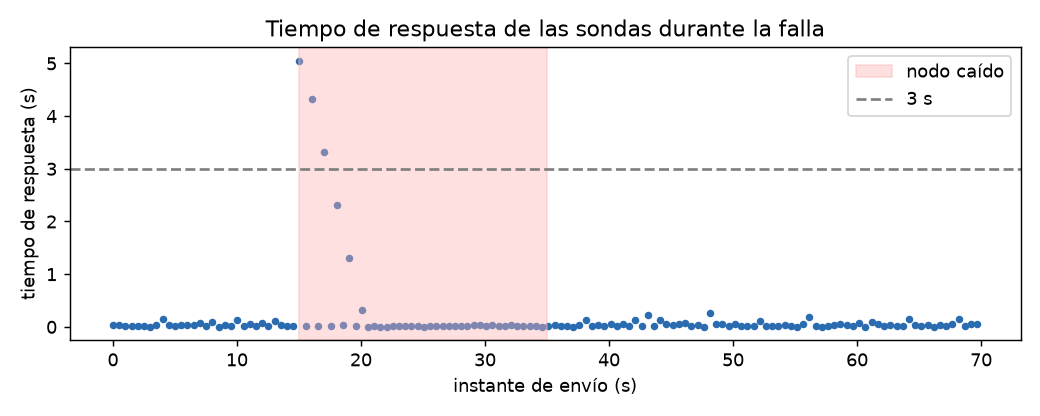
\includegraphics[width=0.9\textwidth]{figuras/disponibilidad.png}
\caption{Tiempo de respuesta de las sondas durante la falla.}
\label{fig:disponibilidad}
\end{figure}

Las sondas enviadas al nodo caído no reciben \texttt{TASK\_ACK}; tras el \emph{timeout} se reasignan a otro nodo y se completan, por eso la disponibilidad es alta pero algunas respuestas tardan alrededor del \emph{timeout} de 5 s.

\subsubsection{Consumo de recursos del nodo coordinador}

\begin{table}[htbp]
\centering
\small
\resizebox{\ifdim\width>\linewidth\linewidth\else\width\fi}{!}{%
\begin{tabular}{|c|c|}
\hline
\textbf{Métrica} & \textbf{Valor} \\ \hline
Mensajes enviados / recibidos & 2124 / 3469 \\ \hline
Tráfico enviado / recibido & 546 KB / 838 KB \\ \hline
Duración & 468 s \\ \hline
Tráfico medio enviado & 1.17 KB/s \\ \hline
Tareas enviadas / completadas / reasignadas / fallidas & 1308 / 1308 / 39 / 0 \\ \hline
\end{tabular}}
\caption{Consumo del nodo que coordinó los experimentos.}
\label{tab:recursos}
\end{table}

\subsubsection{Síntesis de los resultados}

\begin{itemize}
\item \textbf{Descubrimiento:} los nodos se encuentran solos en 0.12 s de media en 5/8 intentos, sin configuración manual.
\item \textbf{Escalabilidad:} con 3 nodos la aceleración fue 1.55$\times$ respecto a un solo nodo.
\item \textbf{Estrategias:} la de menor tiempo total fue Menos cargado.
\item \textbf{Fallos:} la caída se detectó en 4.73 s de media y se completó el 100\,\% de las tareas.
\item \textbf{Disponibilidad:} se completó el 100.0\,\% de las sondas durante la falla de un nodo.
\end{itemize}
